\section{Introduction}
\frame{\tableofcontents[currentsection, hideothersubsections]}

\begin{frame}
\frametitle{Introduction}

\begin{figure}
    \centering
    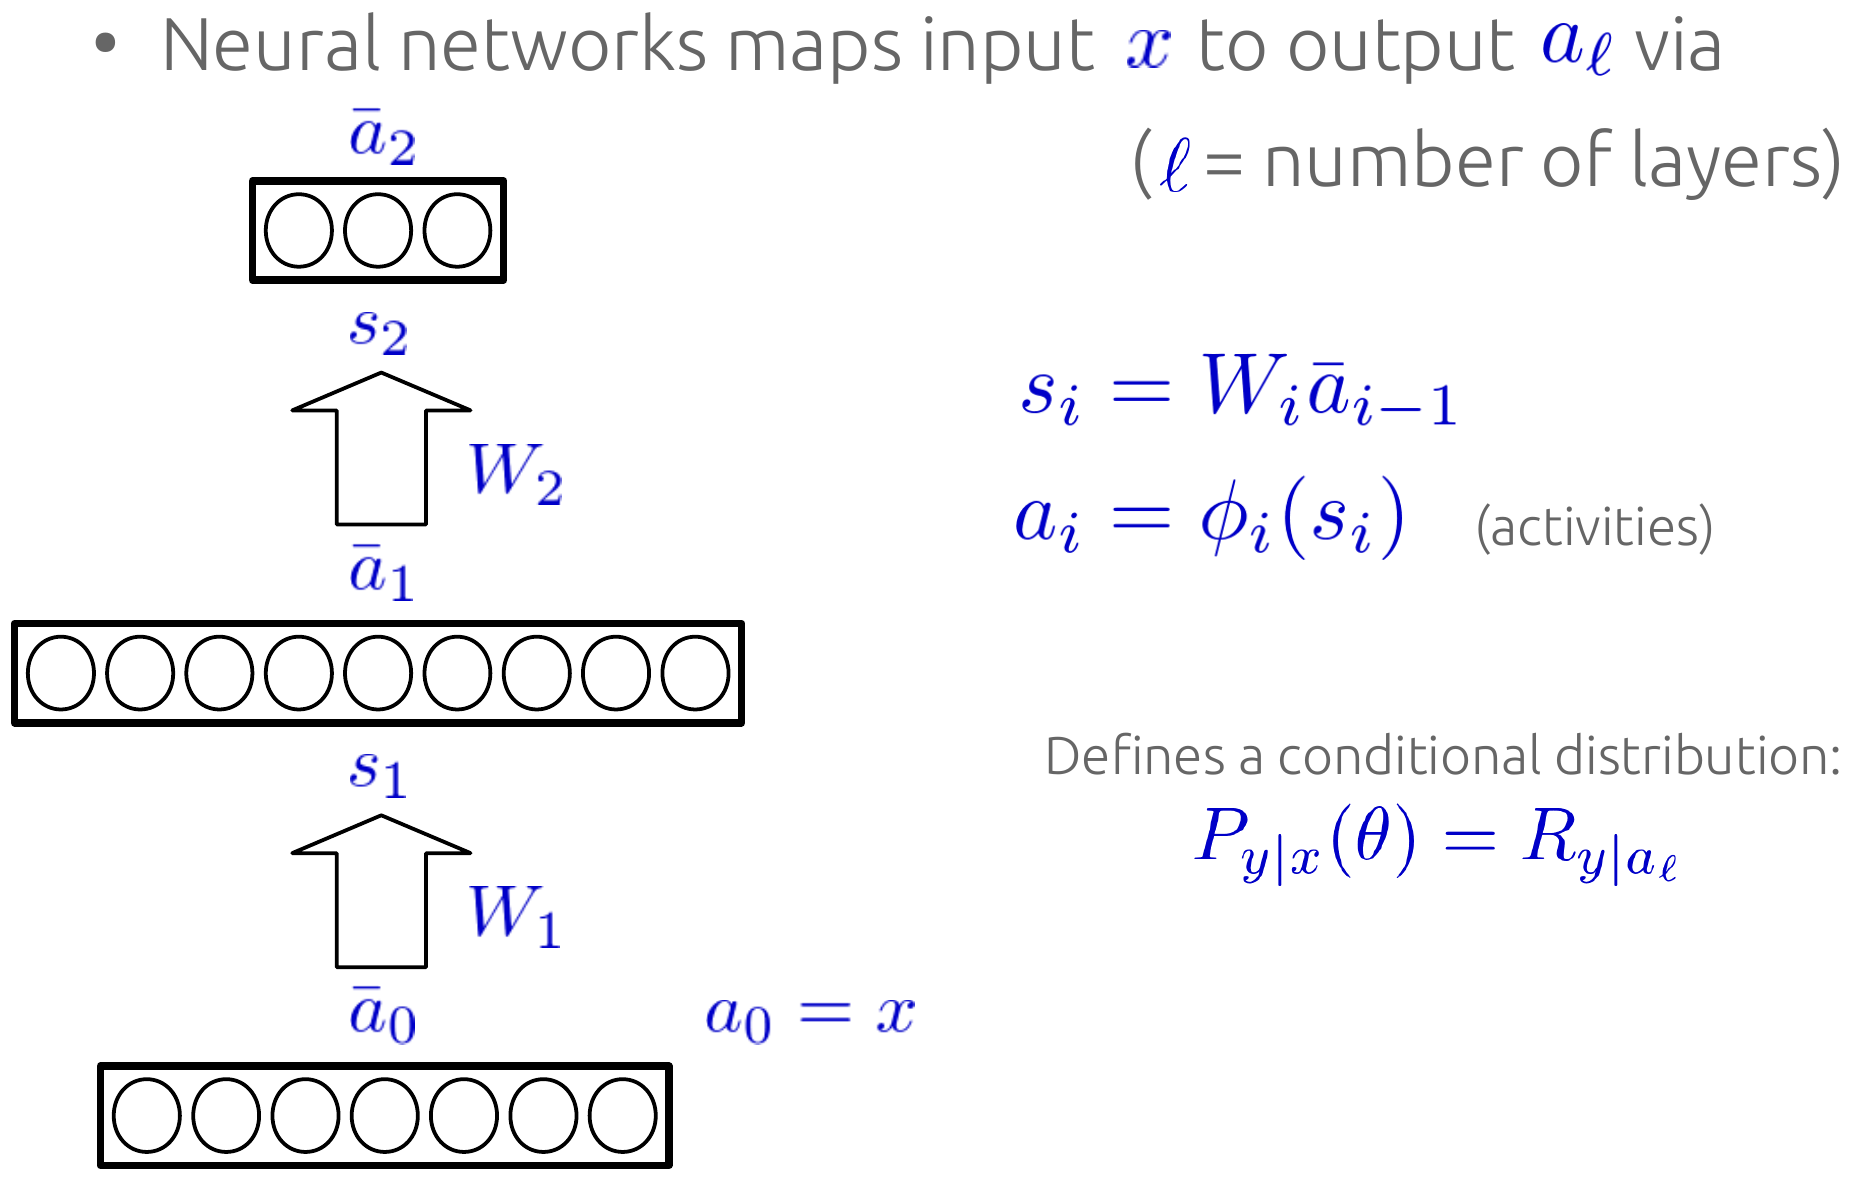
\includegraphics[scale=0.235]{net}
\end{figure}

\end{frame}

\begin{frame}
\frametitle{Introduction}

\begin{figure}
    \centering
    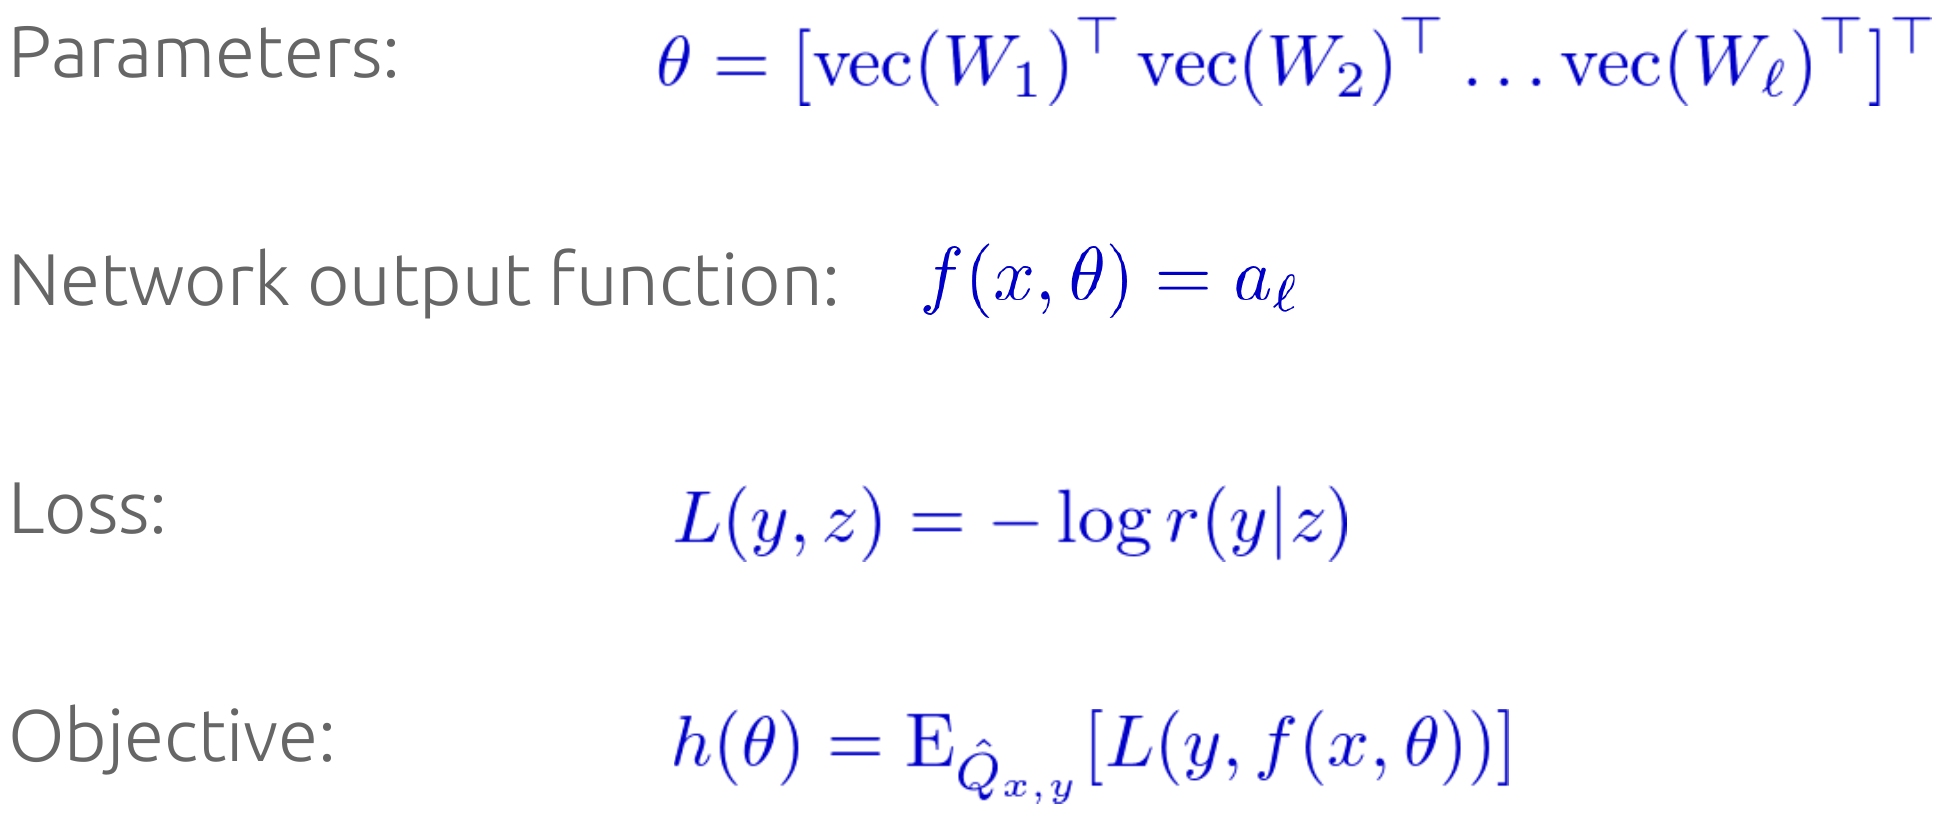
\includegraphics[scale=0.235]{net_param}
\end{figure}

\end{frame}

\begin{frame}
\frametitle{Introduction}

\begin{itemize}
    \item $\bar{a}_i$:\\
        $a_i$ that is appended by a homogeneous coordinate with value 1,
        to capture biar parameters explicitly
    \item $vec$:\\
        an operator that vectorizes matrices by stacking their columns together
    \item $Q_x$:\\
        a data distribution over $x, y$, to which we do not have access,\\
        instead, we use a training distribution over $\hat{Q}_{x, y}$: inputs $x$.
    \item $p(y|x, \theta) = r(y|f(x, \theta))$:\\
        is the density function of $P_{y|x}(\theta) = R_{y|f(x,\theta)}$
\end{itemize}

\end{frame}

%  t, and the model’s predictive dis-
% tribution Py|x (θ) over y
